\section{Planetary Plasma}
Plasma about planetary bodies are infused with magnetic fields. 
For those planetary bodies without intrinsic magnetic fields, crustal magnetic fields such as at Mars and induced magnetic fields caused by the magnetic field lines draping around the planetary body nonetheless are essential to describing particle behavior.
Comets also experience an induced magnetosphere, as confirmed by \textit{in situ} measurements \citep{israelevich1994}.
Although diagrams of the geomagnetic system lend themselves to complexity, the basic particle behavior can be described starting with Newton's Second Law of Motion.


\FloatBarrier
\subsection{Single Particle Motion}
The basic equation of motion for a mass $m$ experiencing a force $\vect{F}$ is
\begin{equation}\label{eq:Feqma}
\vect{F}=m\vect{a} = m \frac{d\vect{v}}{dt}.
%\marginnote{eqn. of motion}
\end{equation}
In the presence of electric field $\vect{E}$, the Lorentz force on a particle with charge $q$ is
\begin{equation}\label{eq:lorentzforceBeq0}
\vect{F} = q\vect{E}.
%\marginnote{Lorentz force, \ensuremath{B\equiv0}}
\end{equation}
In the presence of a magnetic field $\vect{B}$ and electric field $\vect{E}$, a particle at rest will be accelerated and gyrate about $\vect{B}$, driven by the Lorentz force
\begin{equation}\label{eq:lorentzforce}
\vect{F} = q\left(\vect{E} + \vect{v}\times\vect{B}\right).
%\marginnote{Lorentz force}
\end{equation}
The decomposition of \eqref{eq:lorentzforce} into components
\begin{equation}\label{eq:Fperppar}
\vect{F} = \vect{F}_\parallel + \vect{F}_\perp
\end{equation}
where $\vect{F}_\parallel\in \vect{F} \parallel \vect{B}$ and $\vect{F}_\perp \in \vect{F} \perp \vect{B}$\ leads  to the notion that charged particles will gyrate in a magnetic field, with motion along $\vect{B}$ driven by $\vect{E}$ \citep{cravensbook}. 

For simplicity we drop the vector symbol where the context is clear.
The sign of $q$ indicates that positive and negative particles will move in opposite direction for both $F_\parallel$ and $F_\perp$. 
Aurora is observed \citep{borovsky1993} from the solution of~\eqref{eq:Feqma} for particles along $B$
\begin{equation}\label{eq:vpar}
v_\parallel = v_{\parallel,0} + \frac{F_\parallel}{m}t
%\marginnote{\ensuremath{v \parallel B}}.
\end{equation}
The gyroradius
\begin{equation}\label{eq:gyrad}
r_L = \frac{m_s v_\perp}{qB}
%\marginnote{gyroradius}
\end{equation}
and gyrofrequency
\begin{equation}\label{eq:gyfreq}
\Omega_s = \frac{q B}{m_s}
%\marginnote{gyrofrequency}
\end{equation}
follow from solving for 
\begin{equation}\label{eq:vperp}
v_\perp^2 = v_x^2 + v_y^2 
%\marginnote{\ensuremath{v \perp B}}
\end{equation}
with components
\begin{align}
v_x &= v_\perp \cos{\left( \Omega t + \theta \right)} \label{eq:vxy} \\
v_y &= \mp v_\perp \sin{\left( \Omega t + \theta \right)} \nonumber.
\end{align}
The pitch angle
\begin{equation}\label{eq:pitch}
\alpha_p = \tan^{-1}{\frac{v_\perp}{v_\parallel}}
%\marginnote{pitch angle}
\end{equation}
of a particle is the angle between $\vect{v}$ and $\vect{B}$.
As discussed in section~\ref{sec:losscone}, pitch angle is important for determining which particles are most likely to be lost during magnetic mirroring and thereby potentially appearing as aurora.
\FloatBarrier
\subsection{Magnetic Mirroring}\label{sec:mirror}
In general, geomagnetic field lines are not straight. 
The geomagnetic field $B$ converges near Earth and in the magnetotail. 
A significant percentage of the ions and electrons trapped in the geomagnetic field ``mirror''.
Magnetic mirroring here means that $v_\parallel$ changes sign, reversing the direction of particle travel along $B_\parallel$ in the lower magnetosphere and in the magnetotail. 
If via external fields or system reconfiguration a particle's $v_\parallel$ grows significantly enough relative to $v_\perp$, that is, the particle pitch angle \eqref{eq:pitch} decreases, the particle will enter the loss cone and penetrate into the ionosphere.

For a collisionless plasma with slowly changing fields, that is, where the scales of field gradients are small compared to the particle gyroradius, the magnetic moment of the particle \citep{kivelson,chenbook}
\begin{equation}\label{eq:adiabatic1}
\mu = \frac{ m v^2_\perp}{2B}
\end{equation}
remains constant.
When the direction and magnitude of $B$ and $v_\perp$ in \eqref{eq:adiabatic1} change slowly, $\mu$ is the constant known as the first adiabatic invariant. 
Converging $B$-field lines imply $B$ is increasing. 
Since particle mass $m$ is a constant and $\mu$ must remain approximately constant, $v_\perp$ must increase so that $\frac{v^2_\perp}{B}$ remains constant while maintaining a constant
\begin{equation}\label{eq:vcomp}
v = v_\perp + v_\parallel
\end{equation}
since we assume other acceleration sources are negligible.
\eqref{eq:vcomp} and \eqref{eq:adiabatic1} imply that $v_\parallel$ must decrease as $v_\perp$ increases.
Where $\alpha_p \rightarrow \frac{\pi}{2}$ in \eqref{eq:pitch} $v_\parallel \rightarrow 0 $ and the particle mirrors.
For the Earth's ionosphere, electrons mirror with bounce frequency of order \unit[0.1..10]{Hz} and ions mirror with a period of \unit[1..10]{min} \citep{kivelson,newell2009}.
Another implication of \eqref{eq:pitch} with \eqref{eq:adiabatic1} and \eqref{eq:vcomp} and the assumption there is no $E \parallel B$ is that particle kinetic energy
\begin{equation}
W = \frac{1}{2} m v^2 = \frac{1}{2} m \left(v^2_\perp + v^2_\parallel\right)
\end{equation}
is constant, and thereby
\begin{equation}
W_\parallel = W \cos^2 \alpha_p
\end{equation}
and 
\begin{equation}
W_\perp = W \sin^2 \alpha_p.
\end{equation}

%TODO give typical gyrofrequency


\FloatBarrier
\subsection{Loss Cone}\label{sec:losscone}

Assuming a dipolar geomagnetic field, reasonable for altitudes $h < 3 R_E$, the McIlwain L-shell
\begin{equation}\label{eq:Lshell}
L = \frac{r_e}{R_E}
%\marginnote{L-shell number}
\end{equation}
where $r_e$ is the geocentric distance to the point where the $B$ field line crosses the magnetic equator is a convenient parameter for describing near-Earth magnetospheric phenomena.
As L increases, eventually the magnetopause and open field lines are reached leading into the solar wind.
As L decreases, the collisions increase such that the particle behavior becomes collision dominated for small L.
The geocentric distance to a mirroring particle is
\begin{equation}
r=L \cos^2 \lambda
\end{equation}
where $\lambda$ is the magnetic latitude of the field line.
To obtain invariant latitude, that is the magnetic latitude where an L-shell intersects the Earth's surface, plug in $r=R_E, \lambda=\lambda_E, r_0=L R_E$ \citep{kivelson}
\begin{equation}
\Lambda = \cos^{-1} \sqrt{\frac{1}{L}}.
\end{equation}
The particle will be lost if 
\begin{equation}
\alpha_p \leq \sin^{-1}\left(4L^6 - 3 L^5\right)^{-1/4}
\end{equation}
as depicted in the blue area in Figure~\ref{fig:losscone}.
\begin{figure}\centering
	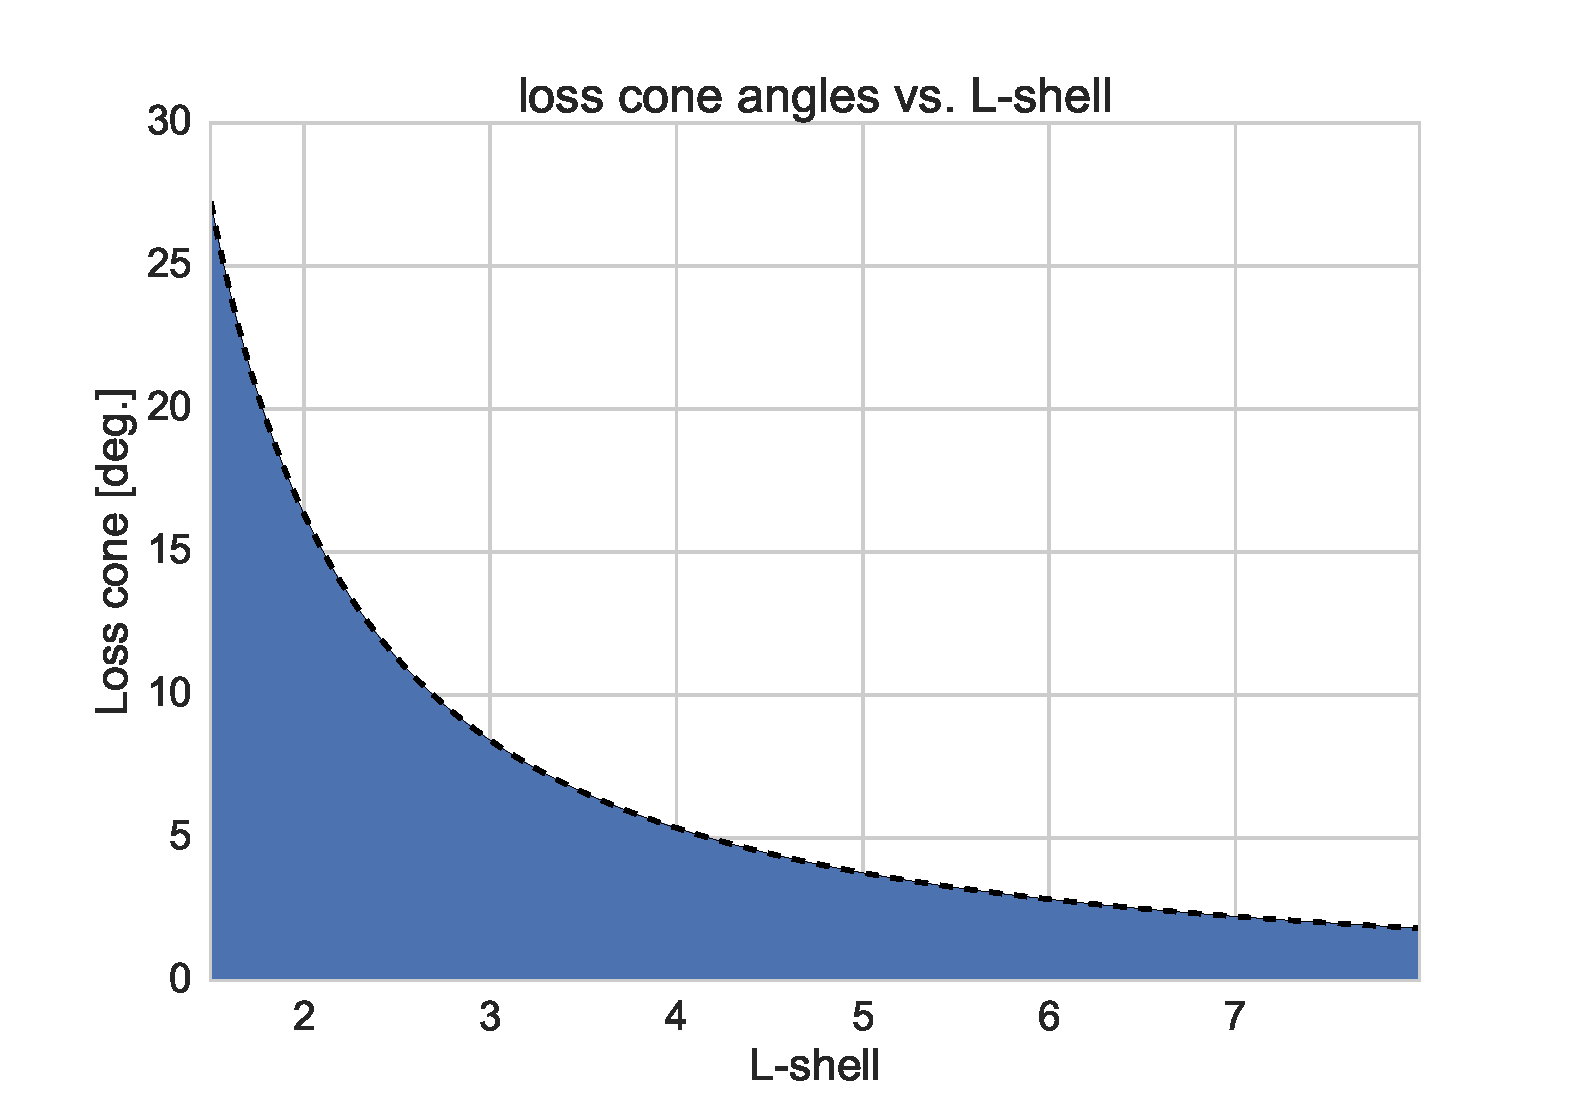
\includegraphics[width=0.8\linewidth]{gfx/lossconeangle}
	\caption{Shaded area indicates loss cone width vs. L-shell}\label{fig:losscone}
\end{figure}
Mirroring particles that are accelerated along $B$ experience an increase in $v_\parallel$ and a decrease in $\alpha_p$, increasing the likelihood the accelerated population will precipitate into the ionosphere and create aurora.
Some important L-shells for Earth are:
\begin{itemize}
	\item nightside plasmapause: 3.5 (active) to 5 (quiet)
	\item inner Van Allen Belt: 1.03 (SAA) to 3
	\item auroral oval: 4..6
\end{itemize}
